\section{Fichier de description de la géométrie}
\label{sec:geom}

\noindent
Ce fichier décrit la géométrie de tête utilisée dans la méthode d'éléments finis surfaciques~: le nombre et le nom des surfaces maillées (interfaces) séparant les différents domaines de
conductivité homogènes ainsi que le nombre et le nom de chacun de ces domaines et leur disposition par rapport aux interfaces.\\ 
Extension du fichier~: *.geom par convention. 

\centerline{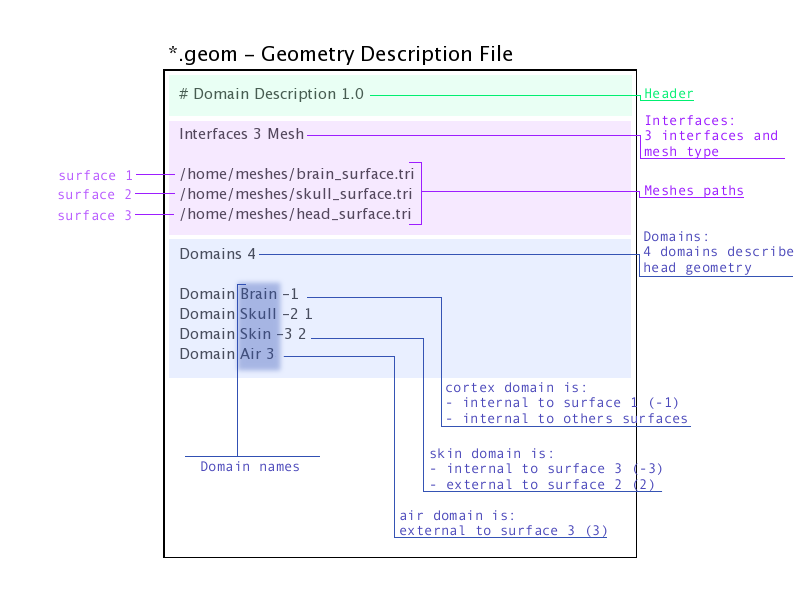
\includegraphics[height=9cm]{geom.png}}

\begin{note}
    Il est conseillé de noter la relation entre domaines et interfaces de la manière
    suivante (noter en premier la référence aux surfaces externes et en deuxième position la surface interne)~:

    \begin{tabular}{ll}
        Domain Brain -1              & \\
        Domain Skull \textbf{1 -2}	 &	\emph{et non pas Domain Skull -2 1} \\
        Domain Skin \textbf{2 -3}	 &	\emph{et non pas Domain Skin -3 2}  \\
        Domain Air 3                 &  \\
    \end{tabular}
\end{note}

\medskip

\begin{note}
    Les "Meshes paths" sont 
    \begin{itemize}
        \item soit absolus (comme le montre le dessin)
        \item soit relatifs à l'endroit où on exécute les lignes de commandes 
    \end{itemize}
    Seuls les formats suivants sont lus pour les surfaces maillées~:
    \begin{itemize}
        \item *.tri~: format TRI issu des premières versions de BrainVisa. Aussi lu par Anatomist.
        \item *.mesh~: format MESH issu des versions 3.0.2 et plus de BrainVisa. Aussi lu par Anatomist.
        \item *.vtk~: format de maillage VTK.
    \end{itemize}
\end{note}

%#############################################################
\section{Fichier de description des conductivités}
\label{sec:cond}

\noindent
Ce fichier décrit les valeurs des conductivités associées aux différents domaines déclarés dans le fichier de description de la
géométrie (section~\ref{sec:geom}).\\ 
Extension du fichier~: *.cond par convention.\\
\warning{bien respecter la casse entre les noms de domaines donnés dans le fichier de description de la géométrie et ceux
notés dans le fichier de description des conductivités !}

\centerline{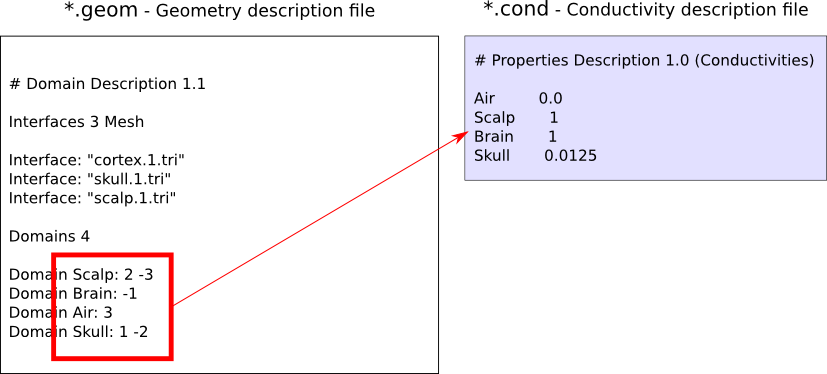
\includegraphics[height=9cm]{cond.png}}



%###################################################

\section{Descriptions des sources d'activité cérébrale}
Les sources sont définies par leur géométrie (position et orientation) et leur amplitude.
OpenMEEG peut traiter deux types de modèles de source: des dipoles isolés, ou bien des dipôles distribués.
Ces deux modèles sont décrits ci-dessous.

%-----------------------------------
\subsection{Position et orientation des sources}
\label{sec:dipoles}
%----
\subsubsection{Dipoles isolés}
\noindent
Les dipoles isolés sont représentés par un fichier texte, dans lequel à chaque ligne correspond un dipôle~: 
\begin{itemize}
    \item les trois premiers nombres (séparés par un espace) sont les coordonnées cartésiennes de la position du dipôle,
    \item les trois derniers nombres (séparés par un espace) sont les coordonnées cartésiennes du vecteur normale donnant
           l'orientation du dipôle.
\end{itemize}
Extension de fichier~: *.dip ou *.txt.

\medskip

\noindent
Exemple d'un fichier décrivant 5 dipôles~:

\centerline{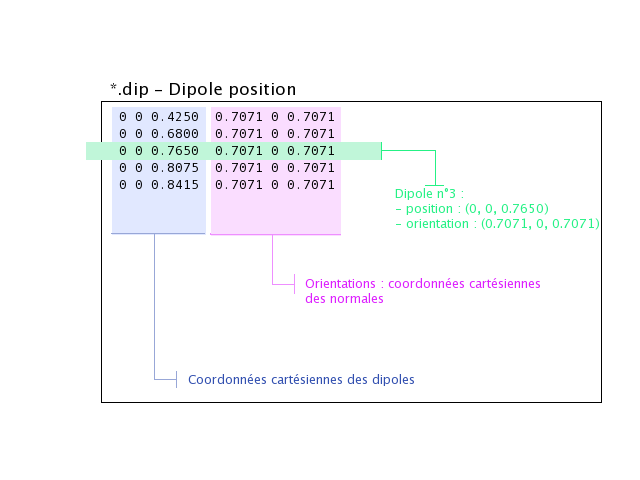
\includegraphics[height=9cm]{dipolePositions.png}}

\begin{note}
    les coordonnées sont définies dans le même repère que celui des maillages (repère de l'IRM en général)
\end{note}

%----
\subsubsection{Distributed dipoles}
Les dipoles distribués sont supportés sur une surface, de format *.tri, *.mesh ou *.vtk. 
%-----------------------------------
\subsection{Activation des sources}
\label{sec:activ}

\noindent
Les fichiers d'activation des sources sont des fichiers texte. A une ligne correspond une source~: 
\begin{itemize}
    \item dans le cas dipolaire, sont écrits sur la ième ligne les états d'activation du ième dipôle,
    \item dans le cas des sources distribuées, sont écrits sur la ième ligne les états d'activation du ième point du maillage
          des sources.
\end{itemize}

\medskip

\noindent
On trouve en colonne les temps auxquels sont associés les activations.

\medskip

\noindent
Exemple dans le cas dipolaire~:

\centerline{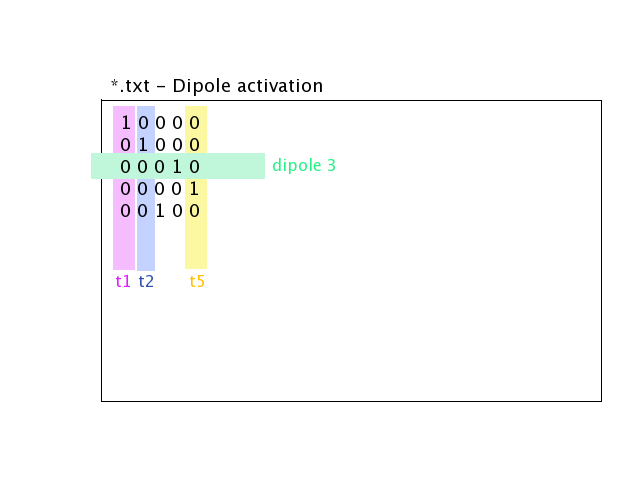
\includegraphics[height=9cm]{dipActiv.png}}

%###################################################

\section{Description des capteurs}
\label{sec:sensors}

\noindent
Les capteurs sont décrits par un fichier texte, dans laquelle chaque ligne contient la position du capteur,
et éventuellement d'autres informations telles que son label ou son orientation. Plus précisément, on dispose de 5 options pour définir les capteurs:
\begin{enumerate}
\item  1 ligne par capteur et 3 colonnes (typiquement pour les électrodes EEG ou des capteurs MEG sans orientation) :
	\begin{itemize}
		\item  les trois colonnes représentent les coordonnées cartésiennes du capteur
	\end{itemize}
\item  1 ligne par capteur et 4 colonnes (typiquement pour les électrodes EEG ou des capteurs MEG sans orientation) :
	\begin{itemize}
		\item   la première colonne contient le nom du capteur (label)
		\item les colonnes 2, 3 et 4  représentent les coordonnées cartésiennes du capteur
	\end{itemize}
\item 1 ligne par capteur et 6 colonnes (typiquement pour des capteurs MEG) :
	\begin{itemize}
		\item  les colonnes 1, 2  et 3  représentent les coordonnées cartésiennes du capteur
		\item  les colonnes 4, 5, et 6 représentent l'orientation du capteur 
	\end{itemize}
\item  1 ligne par capteur et 7 colonnes (typiquement pour des capteurs MEG) :
	\begin{itemize}
		\item la première colonne contient le nom du capteur (label)
		\item les colonnes 2, 3  et 4  représentent les coordonnées cartésiennes du capteur
		\item les colonnes 5, 6, et 7 représentent l'orientation du capteur 
	\end{itemize}
\item 1 ligne par point d'intégration pour chaque capteur, et 8 colonnes (typiquement pour des gradiomètres MEG ou des capteurs réalistes avec bobines) :
	\begin{itemize}
		\item  la première colonne contient le nom du capteur (label)
		\item les colonnes 2, 3  et 4  représentent les coordonnées cartésiennes du capteur
		\item  les colonnes 5, 6, et 7 représentent l'orientation du capteur
		\item  la colonne 8 contient le poids à appliquer pour l'intégration numérique (relative au nom du capteur)
	\end{itemize}

\end{enumerate}

Exemple de description de capteurs MEG:




\centerline{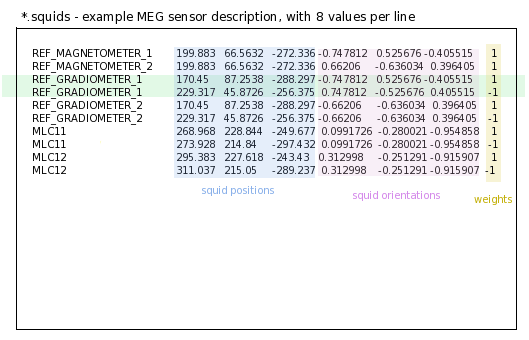
\includegraphics[height=9cm]{sensors-grad.png}}
